\begin{minipage}{9cm}
\section{Equalizer (Ver- \& Entzerrung)}
			$H_v(z)\cdot H_e(z)=1 \longrightarrow H_e(z)=\dfrac{1}{H_v(z)}$\\

			Gilt nicht bei grosser Verz�g., da Entzerrer sonst akausal:\\
			$H_v(z)=H_{vo}(z)\cdot z^{-1} \rightarrow
			 H_e(z)=\dfrac{z^{+1}}{H_{vo}(z)}$

    \end{minipage}
		\hfill
    \begin{minipage}{9cm}    	
			\subsection{Entzerrung von Polen}
			Annahme Rekursiv: $H_v(z)=\dfrac{1}{1+c_1z^{-1}+ \ldots
			+c_nz^{-n}}$\\ 
			FIR-Filter-Entzerrung: $H_e(z)=1+c_1z^{-1}+\ldots+c_nz^{-n}$\\
			
			$H_v(z):$ Verzerrer \hspace{0.5cm} $H_e(z):$ Entzerrer (Equalizer)
    \end{minipage}
		
\vspace{0.25cm}
		
\hrule

	\subsection{Entzerrung von Nullstellen}
    \begin{minipage}{9cm}
		Annahme Verz. travers.: $H_v(z)=1+c_1z^{-1}+\ldots+c_nz^{-n}$\\
		Hauptwert: Wert, bei dem Koeffizient = 1 ist.\\
		Vorl�ufer: Hauptwert ist nicht bei n=0.\\
		Nachl�ufer: Hauptwert ist bei n=0.\\

		\textbf{Rekursive Nachlaufentzerrung (IIR):}\\
		$H_e(z)=\dfrac{1}{1+c_1z^{-1}+\ldots+c_nz^{-n}}$\\
		Stabil wenn $|c_n|<1$ und keine Vorl�ufer\\

		\textbf{Transversale (FIR-) Nachl�uferentzerrung}\\
		$H_e(z)=1+c_{T1}z^{-1}+c_{T2}z^{-2}+\ldots$\\
		Unendlich lange Potenzreihe $\rightarrow$ zeroforcing. Mit beschr�nkter
		Filterl�nge kann gute N�herung erzielt werden.\\
		Bsp.: $H_e(z)=\dfrac{1}{1+az^{-1}}=1-az^{-1}+a^2 z^{-2}-a^3 z^{-3}\ldots$\\

    \end{minipage}
		\hfill
    \begin{minipage}{9cm}    	
		\textbf{Rekursive (IIR) Vorl�uferentzerrung}\\
		Ist nicht sinnvoll, da instabil. Bsp.:\\
		$H_v(z)=a+z^{-1}$ mit $|a|<1$ $\qquad$
		$H_e(z)=\dfrac{z^{-m}}{H_v{z}}=\dfrac{2z^{-m}}{1+2z^{-1}}$\\

		\textbf{Transversale (FIR-) Vorl�uferentzerrung}\\
		$H_v(z)=a+z^{-1}$ mit $|a|<1$\\
		$H_e(z)=\dfrac{z^{-m}}{H_v{z}}=z^{-m}+c_{T(m-1)}z^{-(m-1)}+c_{T(m-2)}z^{-(m-2)}..$\\
		Beispiel f�r $m=3$ Koeffizienten:\\
		$H_e(z)=\dfrac{z^{-3}}{z^{-1}+a} = z^{-2}-az^{-1}+a^2 (-a^3z + a^4z^2+ ..)$\\
		Glieder in Klammer aus Kausalit�tsgr�nden nicht verwenden.\\
    \end{minipage}

\vspace{0.25cm}
		
\hrule

\vspace{0.25cm}

    \begin{minipage}{9cm}
		\subsection{Bsp.: Transvers. FIR-Nullstellenentz.}
		Ziel:\\
		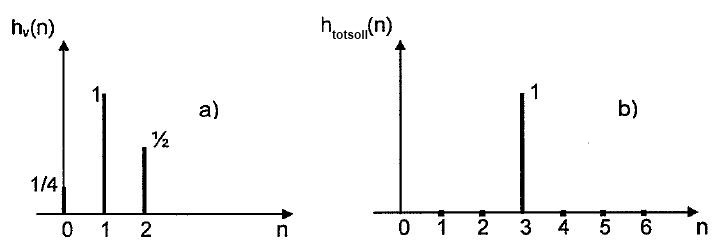
\includegraphics[width=8cm]{./Content/Equalizer/Equalizer01.JPG}
        
        \subsubsection{Zero-Forcing-Method}
        Gleichungssystem f�r die 6 Filterkoeffitienten:\\
        Zu l�sendes Gleichungssystem:\\
				%\begin{alignat}{2}
				%h_{tot}(1)&=c_0+0.25c_1&&=0\nonumber\\
				%h_{tot}(2)&=0.5c_0+c_1+0.25c_2&&=0\nonumber\\
				%h_{tot}(3)&=0.5c_1+c_2+0.25c_3&&=1\nonumber\\
				%h_{tot}(4)&=0.5c_2+c_3+0.25c_4&&=0\nonumber\\
				%h_{tot}(5)&=0.5c_3+c_4+0.25c_5&&=0\nonumber\\
				%h_{tot}(6)&=0.5c_4+c_5&&=0\nonumber
				%\end{alignat}
				\footnotesize
				\vspace{0.25cm}
				
				$\underbrace{\begin{bmatrix}
				1&1/4&0&0&0&0\\
				1/2&1&1/4&0&0&0\\
				0&1/2&1&1/4&0&0\\
				0&0&1/2&1&1/4&0\\
				0&0&0&1/2&1&1/4\\
				0&0&0&0&1/2&1\\
				\end{bmatrix}}_{A_t}\cdot
				\underbrace{\begin{bmatrix}
				c_0\\
				c_1\\
				c_2\\
				c_3\\
				c_4\\
				c_5\\
				\end{bmatrix}}_c=
				\underbrace{\begin{bmatrix}
				0\\
				0\\
				1\\
				0\\
				0\\
				0\\
				\end{bmatrix}}_{h_{totsoll}}$\\
         
				\vspace{0.25cm}
					
    \end{minipage}
		\hfill
    \begin{minipage}{9cm}    	
        \subsubsection{Mean-Square-Method (MSE)}
        FIR-Koeff. durch minimieren der Fehlerquadratsumme errechnen:\\
				
				\textbf{Mittels Extremalstellenmethode (Handrechnung):}\\
				$h_{tot}(n)=h_v(n)*h_e(n)$\\
        $Q=\sum[h_{tot}(n)-h_{totsoll}(n)]^2 \Longrightarrow \frac{\partial Q}{\partial c_i}=0 \Longrightarrow c_i$\\
					
				%\vspace{0.25cm}
        %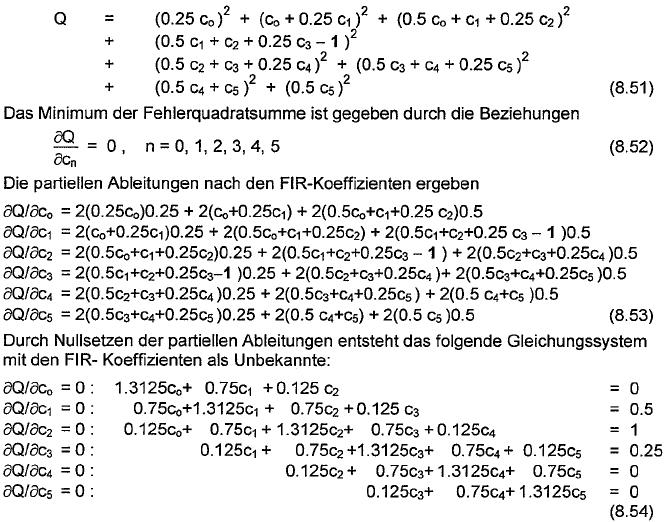
\includegraphics[width=9cm]{./Content/Equalizer/Equalizer02.JPG}\\
       \textbf{ Mittels Matrizenrechnung (MATLAB, Rechner):}\\
				$\scriptsize\underbrace{\begin{bmatrix}
				1/4&0&0&0&0&0\\
				1&1/4&0&0&0&0\\
				1/2&1&1/4&0&0&0\\
				0&1/2&1&1/4&0&0\\
				0&0&1/2&1&1/4&0\\
				0&0&0&1/2&1&1/4\\
				0&0&0&0&1/2&1\\
				0&0&0&0&0&1/2\\
				\end{bmatrix}}_{A_t}\cdot
				\underbrace{\begin{bmatrix}
				c_0\\
				c_1\\
				c_2\\
				c_3\\
				c_4\\
				c_5\\
				\end{bmatrix}}_c=
				\underbrace{\begin{bmatrix}
				0\\
				\textbf{0}\\
				\textbf{0}\\
				\textbf{1}\\
				\textbf{0}\\
				\textbf{0}\\
				\textbf{0}\\
				0\\
				\end{bmatrix}}_{h_{totsoll}}$\\
				
				\vspace{0.25cm}
				
			$c=(A_t^T\cdot A_t)^{-1}\cdot A_t^T\cdot h_{totsoll}$ (Least Mean Square )\\
			
			Die Werte, welche von $h_{totsoll}$ nicht gegeben (frei w�hlbar) sind werden sinnvollerweise als $0$ angenommen.
				
    \end{minipage}

\vspace{0.25cm}
		
\hrule

\vspace{0.25cm}

    \begin{minipage}{9cm}
		\section{Vergleich FIR - IIR}
		\footnotesize
		\begin{tabular}{| p{2cm} | p{2.3cm} | p{2.5cm} |}
            \hline
            Aspekt & FIR & IIR \\
            \hline
            \hline
            Impulsantwort & begrenzt & unbegrenzt \\
            \hline
            Pole/Nullst. & Nur Nullstellen  & Pole u. Nullstellen  
            \\
            \hline
            Stabilit�t & stabil & instabil ausserh. Einheitskr.  
            \\
            \hline
            Hauptwert (1) & beliebig  & am Anfang
            \\
            \hline
            Speicher- u Rechenaufwand & relativ gross & allgemein gering  
            \\
            \hline
            Eignung f�r adapt. Systeme & gut geeignet & nicht geeignet  
            \\
            \hline
            Verz�gerung & $ T_V = \frac12 (N-1) T$ Nur Typ 1 \& 3 & allgemein klein 
            \\
            \hline
        \end{tabular}
 
    \end{minipage}
		\hfill
		\begin{minipage}{9cm}    	
		\section{Wiener Filter}
		Macht optimale Rauschunterdr�ckung mittels minimalem mean square error.\\ \\
		$H(\omega) = \dfrac{\Phi_{XX}(\omega)}{\Phi_{XX}(\omega)+\Phi_{NN}(\omega)}$\\
		\\ $\Phi_{XX}(\omega)$: Leistungsdichtespektrum Signal\\
		$\Phi_{NN}(\omega)$: Leistungsdichtespektrum Rauschen\\
		
    \end{minipage}